\chapter{Virtualization Overhead}
Write about what virtualization overhead is and why it is important in our case ..

Explain how virtualization saves power in the data center by consolidating workloads and how an efficent virtualization mechanism in turn saves power yielding better PUE.

To bring out the virtualization overhead associated with Linux Containers, KVM, and 

\section{Linux Containers}
Refer the notes and th eman pages of LXC for a solid technical discussion on LXC+ Containers

Add a block diagram that shows all the components used in the Linux Containers... cgroups, namespaces, individual filesystems etc..

\begin{figure}[htbp]
\centering
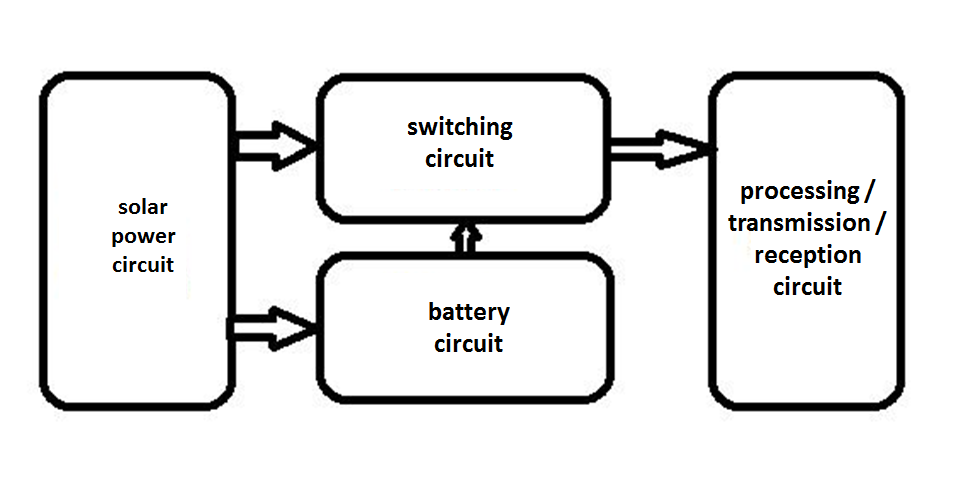
\includegraphics[width=\columnwidth]{block_dia.png}
\caption{Block Diagram of the Mote Platform}
\label{img_blockDia}
\end{figure}


Explain the block diagram in detail.

The device works in two modes:
\begin{enumerate}
\item Solar Powered:
The device performs two tasks in solar powered mode. First, it supplies power to the circuit. Second, it charges the Li-Ion battery.
\item Battery Powered:
The circuit operates in battery powered mode whenever there is insufficient solar power. The circuit uses power from the Li-Ion battery in this mode.
\end{enumerate}

\section{Kernel based Virtual Machines (KVM)}
A good technical discussion on how KVM works ... Refer the papers that already did this .... Add more info. Google it.
Add a nice block diagram of KVM..
\begin{figure}[htbp]
\centering
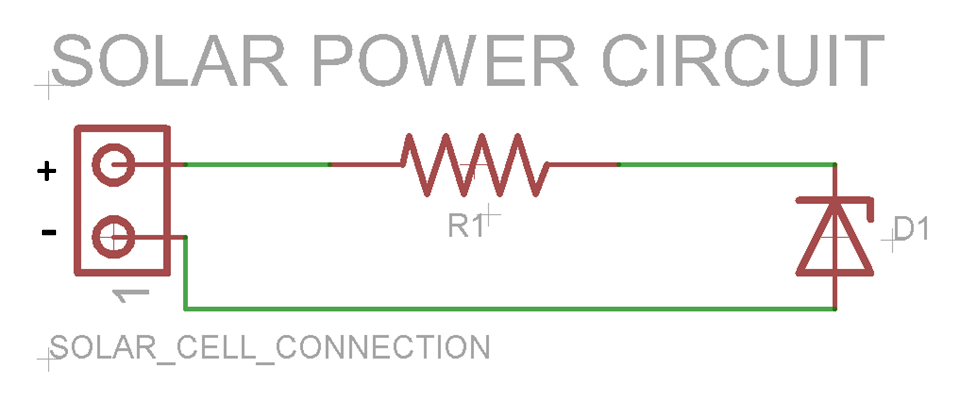
\includegraphics[width=110mm]{solar_pwr_ckt.PNG}
\caption{Solar Power Circuit}
\label{img_solarPowerCircuit}
\end{figure}

As shown in Figure \ref{img_solarPowerCircuit}, Explain the block diagram in detail ..... As shown in Figure \ref{img_solarPowerCircuit}, 


Add more detailed tech discussions ... See anatomy of KVM, Developerworks article by Tim Jones ... 

\begin{tabular}{lllp{10cm}}
where, & • & • & • \\ 
• & $R$ & = & Resistance ($ohms$) \\ 
• & $V_{s}$ & = & Output voltage of solar cell ($volts$) \\ 
• & $V_{z}$ & = & Breakdown voltage of zener diode ($volts$) \\ 
• & $I_{r}$ & = & Amount of current required by circuit ($mA$) \\ 
 &  &  &  \\ 
\end{tabular} 


\section{Xen}

Same as the above two .. A good technical introduction, followed by a block diagram and more detailed explanation.

\begin{figure}[htbp]
\centering
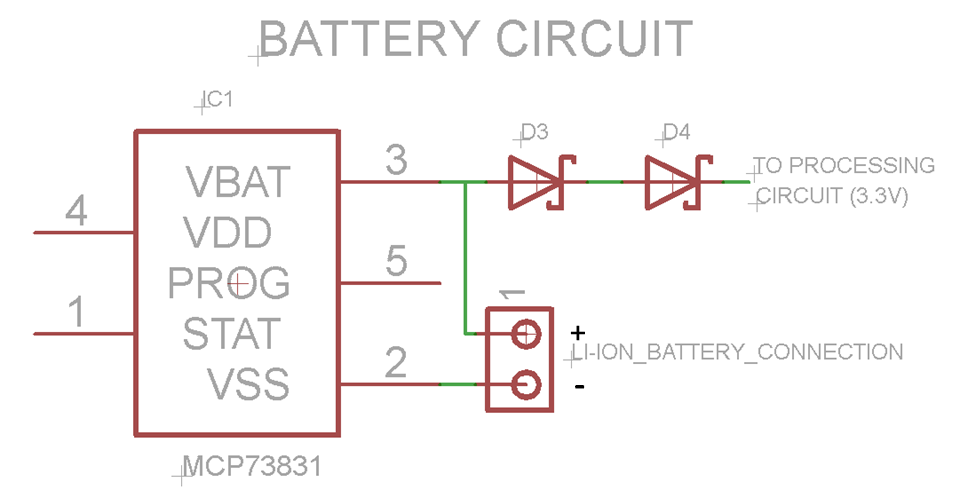
\includegraphics[width=\columnwidth]{battery_ckt.PNG}
\caption{Battery Circuit}
\label{img_batteryCircuit}
\end{figure}

As shown in Figure \ref{img_batteryCircuit}, 